\documentclass[a4paper]{article}

\usepackage[T1]{fontenc}
%\usepackage[utf8]{inputenc}
\usepackage[italian]{babel}
\usepackage{amssymb}
\usepackage{hyperref}
\usepackage{mathtools}
\usepackage{amsthm}
\usepackage[ruled,vlined,noend]{algorithm2e}

%%%%%%%%%%%%%%%%%%%%%%%%%%%%%%%%%%%%
\usepackage{listings} 
\lstdefinestyle{mystyle}{
    breakatwhitespace=false,                   
    captionpos=b,                    
    keepspaces=true,                 
    numbers=left,                    
    numbersep=5pt,                  
    showspaces=false,                
    showstringspaces=false,
    showtabs=False,                  
    tabsize=2
}

\lstset{style=mystyle}

\usepackage{setspace}
\singlespacing
%%%%%%%%%%%%%%%%%%%%%%%%%%%%%%%%%%%%
\usepackage{ulem} 
\usepackage{soul}

\usepackage{graphicx}
\graphicspath{ {./images/} }
%%%%%%%%%%%%%%%%%%%%%%%%%%%%%%%%%%%%
\mathtoolsset{showonlyrefs}  
\hypersetup{
    colorlinks=true,
    linkcolor=black,
    filecolor=black,      
    urlcolor=black,
}

\newcommand{\pluseq}{\mathrel{{+}{=}}}

\newtheorem {theorem}{Theorem}
\newtheorem{corollary}{Corollary}
\newtheorem{lemma}{Lemma}
\newtheorem{remark}{Remark}
\newtheorem{definition}{Definition}

\setcounter{secnumdepth}{3}
\setcounter{tocdepth}{3}

\title{Advanced Programming}
\author{Federico Bruzzone}
%\date{}
\makeindex

\begin{document}
\maketitle
\newpage
% \setlength{\parskip}{0.15em}
\tableofcontents
\setlength{\parindent}{0pt}
\setlength{\parskip}{0.8em}
\newpage

%\section{section}
...

\subsection{subsection}
	
\paragraph{paragraph}

\begin{remark}
    ...
\end{remark}

\subsubsection{subsubsection}

\subsubsection{subsubsection}

\paragraph{paragraph}

\subsection{subsection}
...
\begin{enumerate}
    \item 
    \item
    \item 
\end{enumerate}

\begin{itemize}
	\item 
    \item 
\end{itemize}

\begin{theorem}
    $PO \subseteq NPO$
\end{theorem}
\begin{proof}
    ...
\end{proof}

\begin{equation}
    \begin{aligned}
        \mathit{APX} = \{\Pi | \Pi \mathit{\;di\;ottimizzazione\;t.c.\;}
\exists \rho \geq 1, A, \\\mathit{t.c\;} x\rightarrow A \rightarrow y(x)\;\mathit{con}\;R_\Pi(x, y) \leq \rho\}
    \end{aligned}
\end{equation}


\paragraph{Algoritmo di risoluzione}
L'algoritmo di risoluzione è abbastanza semplice e si basa sulla 
ricerca di un cammino aumentante.

\begin{algorithm}[H]
    \SetAlgoLined
    \KwIn{$G=(V,E)$}
    \KwResult{Matching $M$ per $G$}
     $M \gets \emptyset$\\
     \While{$\Pi = \mathit{findAugmenting(G)}$}{
        $M.update(\Pi)$
     }
     \Return{M}
     \caption{BiMaxMatching}
\end{algorithm}


\subsection{Tecniche greedy}
Nella sezione a seguire si presentano problemi di ottimizzazione per cui 
tecniche greedy funzionano abbastanza bene. 
I problemi affrontati sono quelli di \emph{Load Balancing}, \emph{Center Selection} e \emph{Set Cover}.

\subsubsection{Load balancing}
\label{lb}
Il problema di Load Balancing può essere visto come il compito
di assegnare a macchine dei lavori da compiere, che richiedono del tempo, 
in modo da minimizzare il tempo totale.


\begin{theorem}
    Load Balancing è NPO completo
\end{theorem}
Bisogna perciò trovare un modo di approssimare una soluzione.
\paragraph{Greedy balance}
Il primo approccio alla risoluzione del problema è quello di assegnare la prossima
task alla macchina più scarica in questo momento.

\begin{algorithm}[H]
    \SetAlgoLined
    \KwIn{$M$ numero di macchine, $t_0, \dots, t_n$ task}
    \KwResult{Assegnamento delle task alle macchine}
     $L_i \gets 0\;\forall i \in M$\\
     $\alpha \gets \emptyset$\\
     \For{$j = 0, \dots, n$}{
         $\hat{i} = \min(L_i)$\\
         $\alpha(j) = \hat{i}$\\
         $L_{\hat{i}} \pluseq t_j$
     }
     \Return{$\alpha$}
     \caption{GreedyBalance}
\end{algorithm}

\begin{lstlisting} %[language=Python, caption=Python example]

import numpy as np
    
def incmatrix(genl1,genl2):
    m = len(genl1)
    n = len(genl2)
    M = None #to become the incidence matrix
    VT = np.zeros((n*m,1), int)  #dummy variable
    
    #compute the bitwise xor matrix
    M1 = bitxormatrix(genl1)
    M2 = np.triu(bitxormatrix(genl2),1) 

    for i in range(m-1):
        for j in range(i+1, m):
            [r,c] = np.where(M2 == M1[i,j])
            for k in range(len(r)):
                VT[(i)*n + r[k]] = 1;
                VT[(i)*n + c[k]] = 1;
                VT[(j)*n + r[k]] = 1;
                VT[(j)*n + c[k]] = 1;
                
                if M is None:
                    M = np.copy(VT)
                else:
                    M = np.concatenate((M, VT), 1)
                
                VT = np.zeros((n*m,1), int)
    
    return M
\end{lstlisting}

%%%%%%%%%%%%%%%%%
\usepackage{listings}
\usepackage{xcolor}

\definecolor{codegreen}{rgb}{0,0.6,0}
\definecolor{codegray}{rgb}{0.5,0.5,0.5}
\definecolor{codepurple}{rgb}{0.58,0,0.82}
\definecolor{backcolour}{rgb}{0.95,0.95,0.92}

\lstdefinestyle{mystyle}{
    backgroundcolor=\color{backcolour},   
    commentstyle=\color{codegreen},
    keywordstyle=\color{magenta},
    numberstyle=\tiny\color{codegray},
    stringstyle=\color{codepurple},
    basicstyle=\ttfamily\footnotesize,
    breakatwhitespace=false,         
    breaklines=true,                 
    captionpos=b,                    
    keepspaces=true,                 
    numbers=left,                    
    numbersep=5pt,                  
    showspaces=false,                
    showstringspaces=false,
    showtabs=false,                  
    tabsize=2
}

\lstset{style=mystyle}
\section{}

\subsection{Informazioni generali}

\textbf{Scopo del corso}
\begin{itemize}
	\item Scoprire il concetto di separazione dei compiti;
	\item Imparare a programmare decomponendo le funzionalità del SW;
	\item Imparare ad ottimizzare il SW separandone le funzionalità;
	\end{itemize}
\textbf{Materiale di riferimento}
\begin{itemize}
	\item i licidi del corso;
	\item Ira R. Forman and Note B. Forman. Java Reflection in Action Manning Publications, October 2004;
	\item Ramnivas Laddad. AspectJ in Action: Pratical Aspect-Oriented Programming. Manning Pubblications Company, 2003;
\end{itemize}



















\subsubsection{How to use Python}	
\textbf{We are condidering Python 3+}
\begin{itemize}
	\item version > 3 is incompatible with previus version;
	\item version 2.7 is the current version.
\end{itemize}
\textbf{A python program can be:}
\begin{itemize}
	\item edited in the python shell and executed step-by-step by the shell;
	\item edited and run through the iterpreter.
\end{itemize}

\subsection{Overview of the Basic Concepts}	

\subsubsection{Our first Python program}
\hrule
\begin{lstlisting}[language=Python, caption=humanize.py]
SUFFIXES = {1000: ['KB', 'MB', 'GB', 'TB', 'PB', 'EB', 'ZB', 'YB'], 
            1024: ['KiB', 'MiB', 'GiB', 'TiB', 'PiB', 'EiB', 'ZiB', 'YiB']}
def approximate_size(size, a_kilobyte_is_1024_bytes=True):
	''' Convert a file size to human-readable form. '''
	if size < 0:
		raise ValueError('number must be non-negative')
	multiple = 1024 if a_kilobyte_is_1024_bytes else 1000
	for suffix in SUFFIX[multiple]:
		size /= multiple
		if size < multiple:
			return '{0:.1f} {1}'.format(size, suffix)
		raise ValueError('number too large')
				
if __name__ == '__main__':
	print(approximate_size(1000000000000, False))
	print(approximate_size(1000000000000))
\end{lstlisting}
\hrule	

\subsubsection{Declaring function}	
\textbf{Python has function}
\begin{itemize}
	\item no header files à la C/C++;
	\item no interface/implementation à la Java.
\end{itemize}			
\hrule
\begin{lstlisting}[language=Python]
def approximate_size(size, a_kilobyte_is_1024_bytes=True):
\end{lstlisting}	
\begin{enumerate}
	\item \textbf{def}: function definition keyword;
	\item \textbf{approximate\_size}: function name;
	\item \textbf{a\_kilobyte\_is\_1024\_bytes}: comma separate argument list;
	\item \textbf{=True}: default value.
\end{enumerate}
\hrule		
\textbf{Python has function}
\begin{itemize}
	\item no return type, it always return a value (\textbf{None} as a default); 
	\item no parameter types, the interpreter figures out the parameter type.
\end{itemize}	

\subsubsection{Calling Functions}
\textbf{Look at the bottom of the \textit{humanize.py} program}
\hrule
\begin{lstlisting}[language=Python]
if __name__ == '__main__':
	print(approximate_size(1000000000000, False))
	print(approximate_size(1000000000000))
\end{lstlisting}
\begin{enumerate}
	\item[2] in this call to \textbf{approximate\_size()}, the \textbf{a\_kilobyte\_is\_1024\_bytes} parameter will be \textbf{False} since you explicitly pass it to the function;
	\item[3] in this row we call  \textbf{approximate\_size()} with only a value, the parameter \textbf{a\_kilobyte\_is\_1024\_bytes} will be \textbf{True} as defined in the function declaration.
\end{enumerate}
\hrule
\textbf{Value can be passed by name as in}:
\hrule
\begin{lstlisting}[language=Python]
def approximate_size(a_kilobyte_is_1024_bytes=True, size=1000000000000)
\end{lstlisting}	
\hrule
\textbf{Parameters' order is not relevant}

\subsubsection{Writing readable code}
\textbf{Documentation Strings}
A python function can be documented by a documentation string (docstring for short).
\begin{center}
	\textit{''' Convert a file size to human-readable form.  '''}
\end{center}
\textbf{Triple quotes delimit a single multi-string}
\begin{itemize}
	\item if it immediatly follows the function's declaration it is the doc-string associated to the function;
	\item docstrings can be retrieved at run-time (they are attributes).
\end{itemize}
\textbf{Case-Sensitive}
All names in Python are case-sensitive

\subsubsection{Everything is an object}
\textbf{Everything in Python is an object, functions included}
\begin{itemize}
	\item \textbf{import} can be used to load python programs in the system as modules;
	\item the dot-notation gives access to the the public functionality of the imported modules;
	\item the dot-notation can be used to access the attributes (e.g., the \textbf{\_\_doc\_\_})
	\item \textbf{humanize\.approximate\_size.\_\_doc\_\_} gives access to the docstring of the \textbf{approximate\_size()} function; the docstring is stored as an attribute.
\end{itemize}

\subsubsection{Everything is an object (Cont'd)}
\textbf{In python is an object, better, is a \textbf{first-calss object}}
\begin{itemize}
	\item everything can be assigned to a variable or passed as an argument
\end{itemize}
\hrule
\begin{lstlisting}[language=Python]
h1 = humanize.approximate_size(9128)
h2 = humanize.approximate_size
\end{lstlisting}	
\begin{itemize}
	\item \textbf{h1} contains the string calculated by \textbf{approximate\_size(9128};
	\item \textbf{h2} contains the "function" object \textbf{approximate\_size()}, the result is not calculated yet;
	\item to simplify the concept: \textbf{h2} can be considered as a new name of (alias to) \textbf{approximate\_size}.
\end{itemize}
\hrule

\subsubsection{Indenting code}
\textbf{No explicit block delimiters}
\begin{itemize}
	\item the only delimiter is a column (':') and the code indentation;
	\item code blocks (e.g., functions, if statements, loops, ...) are defined by their indentation;
	\item white spaces and tabs are relevant: use them consistently;
	\item indentation is checked by the compiler.
\end{itemize}

\subsubsection{Exceptions}
\textbf{Exceptions are Anomaly Situations}
\begin{itemize}
	\item C encourages the use of return codes which you check;
	\item Python encourages the use of exceptions which you handles.
\end{itemize}
\textbf{Raising Exceptions}
\begin{itemize}
	\item the \textbf{raise} statement is used to rise an exception as in:
\begin{lstlisting}[language=Python]
raise ValueError('number must be non-negative')
\end{lstlisting}
	\item syntax recalls function calls: \textbf{raise} statement followed by an exception name with an optional argument;
	\item exceptions are relized by classes.
\end{itemize}
\textbf{No need to list the exceptions in the function declaration handling Exceptions}
\begin{itemize}
	\item an exception is handled by a \textbf{try} ... \textbf{except} block.
\hrule
\begin{lstlisting}[language=Python]
try:
	from lxml import etree
except ImportError:
	import xml.etree.ElementTree as etree
\end{lstlisting}
\hrule
\end{itemize}

\subsubsection{Running scripts}
\textbf{Look again, at the bottom of the \textit{humanize.py} program}:
\hrule
\begin{lstlisting}
if __name__ == '__main__':
	print(approximate_size(1000000000000, False))
	print(approximate_size(1000000000000))
\end{lstlisting}
\hrule
\textbf{Modules are Objects}
\begin{itemize}
	\item they have a built-in attribute \textbf{\_\_name\_\_}
\end{itemize}
\textbf{The value of \textbf{\_\_name\_\_} depends on how you call it}
\begin{itemize}
	\item if imported it contains the name of the file without path and extension.
\end{itemize}

\section{Computational Reflection}

\subsection{Computational Reflection}

\subsubsection{A first definition}

Computational reflection can be intuitively defined as:

\textit{"The activity done by a SW system to represent and manipulate its own structure and behavior"}

The reflective activity is done analogously to the usual system activity

\subsection{Reflection}

\subsubsection{Historical Overview}

\textbf{In the sisties}
\begin{itemize}
	\item Research field: artificial intelligence;
	\item First approaches to relection: intelligent behavior;
\end{itemize}

\textbf{In the eighties}
\begin{itemize}
	\item Research filed: programming languages;
	\item Brian C. Smith, he introduces the reflection in Lisp (1982 and 1984), the reflective tower has been defined;
	\item Several reflective list-oriented languages have been defined (they exploit the quoting machanism);
\end{itemize}

\textbf{In the meanwhile}
\begin{itemize}
	\item Research field: logic programming;
	\item the meta-programming takes place in PROLOG;
\end{itemize}

\textbf{Between the eighties and the nineties}
\begin{itemize}
	\item Research fild: object-oriented programming languages;
	\item Pattie maes defines the computational reflection in OOPL (1987);
	\item Several people move from Lisp to OO:
		\begin{itemize}
			\item P. Coite, ObjVLips (1987)
			\item A. Yonezawa, ABCL-R (1988)
			\item J. des Rivières e G. Kiczales MOP for CLOS (1991)
		\end{itemize}
	\item SmallTalk is elected as the best reflective programming language
\end{itemize}

\textbf{In te nineties}
\begin{itemize}
	\item Research field: typed and/or compiled object-oriented programming languages;
	\item Shigeru Chiba realizes OpenC++ (1993-1995), OpenJava (1999);
\end{itemize}

\textbf{In the 1997}
\begin{itemize}
	\item Gregor Kiczales et al. defined the aspect-oriented programming and the story ends;
\end{itemize}

\subsection{Computational Reflection}

\subsubsection{Reflection à la Pattie Maes}

\textbf{Pattie Maes has pioneered the filed}
\begin{itemize}
	\item a \textbf{computational system} is a system that can reason about and act on its applicative somain;
	\item a computational system is \textbf{causally connected} to its domain if and only if a change to its domain is reflected on it and vice versa;
	\item a \textbf{meta-system} is a computational system whose applicative domain in another computational system;
	\item \textbf{reflection} is the property of reasoning about and acting on itself;
\end{itemize}

\textbf{therefore}
\begin{itemize}
	\item a \textbf{reflective system} is a meta system causally connected to itself;
\end{itemize}

\subsubsection{Reflective system}

\textbf{From the definition, we can evince that a reflective system is:}
\begin{itemize}
	\item a software system logically layered into two or more levels respectively called base-level and meta-levels;
	\item the system running in a meta-level observes and manipulates the system running in the underlying level (reflective tower);
\end{itemize}

\textbf{Characteristics}
\begin{itemize}
	\item the system running in the base-level is unaware of the existence and of the work of the systems running in the overlying levels;
	\item a meta-level system acts on a representation (called the system running in the underlying levels; and
	\item a system and its reification are causally connected and therefore, they are kept mutually consistent
\end{itemize}

\subsubsection{Reflective system: Base- and Meta-levels}

\textbf{A meta-level system refies what it is implicit (e.g. mechanisms and structure) of the underlying base- or meta-level}

\subsubsection{How to Characterize a Reflective System}

\textbf{The reflective systems can be classified based on:}
\begin{itemize}
	\item what and when
\end{itemize}

\textbf{What kind of reflective actions the system can carry out:}
\begin{itemize}
	\item structural and behavioral reflection;
	\item introspection (just to observe) and intercession (to alter)
\end{itemize}

\textbf{When the meta-level entities exist:}
\begin{itemize}
	\item compile-time
	\item load-time; and
	\item run-time
\end{itemize}

\subsubsection{Behavioral and structural reflection}

\textbf{The behavioral reflection allows the program of monitoring and manipulating its own computation, e.g.:}
\begin{itemize}
	\item to trap a method call and activating a different method instead;
	\item to monitor the object state;
	\item to create new objects, and so on
\end{itemize}

\textbf{These activities can take place at run-time without a specific support}

\textbf{The structural reflection allows the program of inspecting and altering its own structure, e.g.:}
\begin{itemize}
	\item the code of a method can be modified or removed from the class;
	\item new methods and field can be added to a class, and so on;
\end{itemize}

\textbf{These activities need a specific support by the execution environment (from the VM, RTE, ...) to be carried out at run-time}

\subsubsection{Reification}
\textbf{The base-level entities (referents) are reified into the metalevel, i.e., they have a representative into the meta-level}

\textbf{Such a representative, called reification, has to:}
\begin{itemize}
	\item support all the operations and have the same characteristics of the corresponding referent;
	\item be kept consistent to its referent ( causal connection);
	\item be subjected to the manipulations of the meta-level entities to protect the base-level entities from potential inconsistency
\end{itemize}

\textbf{Any change carried out on the reification has to be reflected on the corresponding referent.}

\subsection{To Develop a Reflective System}
\textbf{Jacques Ferber [2] has raised some issues that the developers must take in consideration:}
\begin{itemize}
	\item which kind of entities should be reified?
	\item what and how it is implemented the causal connection?
	\item when does the execution shift to the meta-level?
\end{itemize}

\subsection{Which Kind of Entities Should Be Reified?}
\textbf{It depends on the programming language:}
\begin{itemize}
	\item functional: lambda expression/closures, environment, continuations, and so on ...;
	\item object-oriented: objects, methods, classes, messages and so on ...;
	\item concurrent and object-oriented: threads, processes, schedulers, monitors, and so on ...;
	\item distribution: namespaces, proxies, mailers, and so on ...
\end{itemize}

\subsection{What and How It Is Implemented the Causal Connection?}
\textbf{It depends on when the reflective activities take place:}
\begin{itemize}
	\item atrun-time: the causal connection is explicit and must be maintained by an entities super-parties, e.g., by the virtual machine or by the run-time environment;
	\item at compile-time: the causal connection is implicit, base-level and meta-levels are merged together during a preprocessing phase;
	\item at load-time: in this case the causal connection behaves as in the case, reflection takes place at compile-time;
\end{itemize}

\textbf{Most of the times, the supported reflective activity is related to observe (introspection) the base-level system so the causal connection become unilateral and can be managed by the metaentities.}

\subsection{When Does the Execution Shift to the Meta-Level?}
\textbf{Switching among levels depends on:}
\begin{itemize}
	\item which entities are reified;
	\item when such entities are reified; and
	\item how the causal connection is managed
\end{itemize}

\textbf{The shift-up and-down actions}
\begin{itemize}
	\item the shift-up and-down actions.
\end{itemize}

\textbf{When}
\begin{itemize}
	\item an observed element changes; or
	\item an action is going to be done;
\end{itemize}

\textbf{the computational flow passes into the meta-level (shift-up)}

\textbf{Instead}
\begin{itemize}
	\item the computational flow goes back (shift-down) on the meta-level program decision
\end{itemize}

\textbf{Usually, the shift-up action is managed by call-backs}

\section{Reflection in OO Programming Languages}

\subsection{Structural and Behavioral Reflection}

\textbf{Structural Reflection}
\begin{itemize}
	\item Object creation and init
		\begin{itemize}
			\item constructor
			\item prototype
			\item meta-classes
		\end{itemize}
	\item Class manipulation
		\begin{itemize}
			\item to add or remove fields
			\item to add or remove methods
			\item to change the super class
		\end{itemize}
\end{itemize}

\textbf{Behavioral Reflection}
\begin{itemize}
	\item message sending
		\begin{itemize}
			\item classes and inheritance
			\item prototypes and delegation
			\item errors
			\item encapsulations
			\item proxies
			\item meta-objects
		\end{itemize}
\end{itemize}

\subsection{Structural Reflection}
The objects running in the meta-level, called \textbf{meta-objects} are associated to all (or just to some of) the objects running in the base-level, called \textbf{referents}.

The connection among referents and meta-objects is called \textbf{causal connection} when it is a two-way link or \textbf{meta-connection} when it is a one-way link.

The meta-objects exist at run-time and extend or modify the semantics of some mechanisms:

-  method invocation, field access, object creation, and so on

The \textbf{MOP} is the set of messages that a meta-object can understand

\subsubsection{Es.To Enrich the Behavior of a Method Call}

\begin{center}
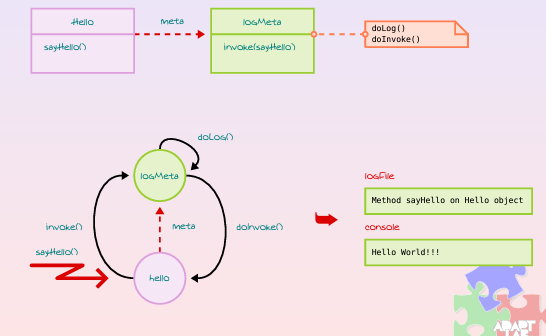
\includegraphics[scale=0.7]{1-To-Enrich-the-Behavior-of-a-Method-Call}
\end{center}

\subsubsection{Different views}

\begin{center}
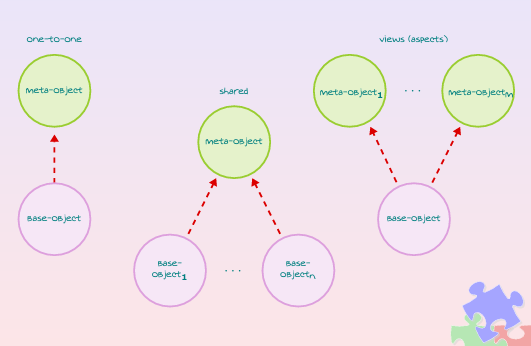
\includegraphics[scale=0.7]{2-different-views}
\end{center}

\subsubsection{Classes as meta objects}

\begin{center}
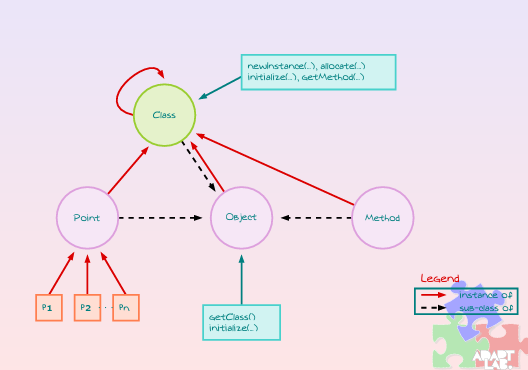
\includegraphics[scale=0.7]{3-classes-as-meta-objects}
\end{center}

\subsubsection{Classes AS Meta-Objects (Cont'd)}
\textbf{The meta-class based approach}
\begin{itemize}
	\item the classes carry out there flective activity
	\item the reflective tower is realized by the inheritance link
\end{itemize}

\textbf{Drawbacks}
\begin{itemize}
	\item all the instances of a classs hare the same meta-class therefore the same reflective behavior (the granularity of reflection is at the class level)
	\item the classes have to be available a trun-time
\end{itemize}

\textbf{Programming Languages}
\begin{itemize}
	\item SmallTalk (Adele Goldberg,1972)
	\item ObjVLisp (PierreCointe,1987)
	\item IBMSystemObjectModel (IBM,1992)
\end{itemize}

\subsubsection{Classes AND meta objects}

\begin{center}
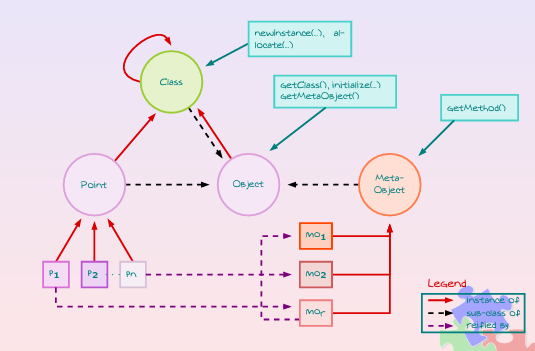
\includegraphics[scale=0.7]{4-classes-and-meta-objects}
\end{center}

\subsubsection{Classes AND Meta-Objects (Cont'd)}
\textbf{The meta-class based approach}
\begin{itemize}
	\item some special objects instantiated by a special class are associated to the base-level objects, they deal with the reflective computation
	\item the reflective tower is realized by clientship
\end{itemize}

\textbf{Drawback and Benefits}
\begin{itemize}
	\item the granularity of reflection is at the object level
	\item it cannot manage object communications, the approach lacks of a global view of the communication
\end{itemize}

\textbf{Programming Languages}
\begin{itemize}
	\item CCEL(Carolyn Duby, 1992), Iguana (Brendan Gowing and Vinny Cahill, 1996);
	\item ABCL-R (Akinori Yonezawa and Satoshi Matsuoka, Actors meet Reflection, 1988);
	\item OpenC++ (Shigeru Chiba < 2.0, 1993)
\end{itemize}

\subsubsection{Reification of the communication}

\begin{center}
\includegraphics[scale=0.7]{5-reification-of-communication}
\end{center}

\subsubsection{Classes AND Meta-Objects (Cont'd)}
\textbf{Approach to the reification of the communication}
\begin{itemize}
	\item some special objects reify the messages exchanged among the baselevel objects, these special objects deal with the reflective computation.
\end{itemize}

\textbf{Drawback and Benefits}
\begin{itemize}
	\item the granularity of reflection is at the level of method call (very flexible)
	\item it is possible to reflect on the whole message exchange (global view)
	\item there is a meta-entities proliferation; and
	\item the lifecycle of the meta-entities is strictly tied to the lifecycle of the message exchange (lost the history of the reflective computation)
\end{itemize}

\textbf{Programming Languages}
\begin{itemize}
	\item Mering (Jacques Ferber, 1987)
	\item  CodA (Jeff McAffer, 1994), mChaRM (Walter Cazzola, 2001)
\end{itemize}

\subsubsection{Conclusion}
\textbf{Computational Reflection}
\begin{itemize}
	\item It permits to open up a system to postpone some decisions
	- the same philosophy adopted by the late-binding mechanism.
	\item it depends on the awareness that a system have of itself
	- strictly related to the “self” of the object-oriented programming languages
	\item it specializes some of the object-oriented basic mechanisms (constructors, invocations, and so on)
	- it exploits the classic mechanisms: inheritance, delegation
\end{itemize}

\textbf{Its use produces a better comprehension of the object-oriented mechanism and of their implementation}





\section{Meta-object Protocol and Separation of concerns}

\subsection{Open Implementation \& Meta-Object Protocol}

\subsubsection{Introduction}
"The work presented in this book is based ona \textbf{simple intuition}:

if \textbf{substrate systems} like programming languages, object
the details of the implementation of the base-level system are open
up to the meta-level system.
systems, databases or operating systems can \textbf{be tailored} to

meet particular application needs as they arise,

rather than having \textbf{to hack around} existing deficiencies,

application writers are better of."

Cit. Gregor Kiczales and Andreas Pæpcke

\subsubsection{System Awareness}
The computational reflection allows a system of observing and manipulating its components

\textbf{In particular}
\begin{itemize}
	\item the meta-level entities observe and manipulate the base-level entities, and
	\item these are NOT aware of being observed and manipulated.
\end{itemize}

\textbf{Therefore}:
\begin{itemize}
	\item there is a “black-box” use of the functionality of the base-level system
	\item the behavior of the base-level system and its structure can be dynamically modified, and
	\item the details of the implementation of the base-level system are open up to the meta-level system
\end{itemize}

\subsubsection{Black- and Gray-Box Approaches}

\begin{center}
%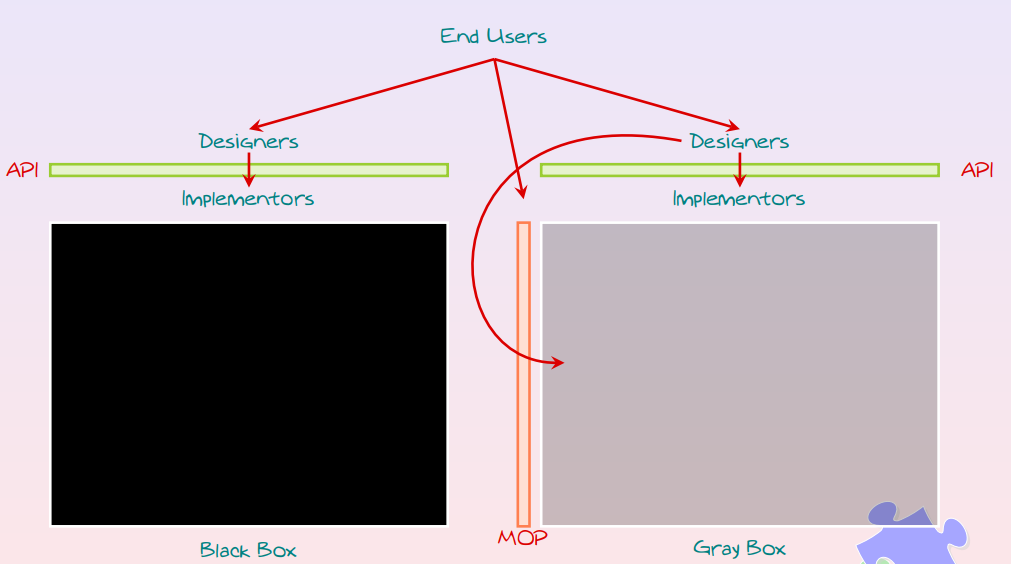
\includegraphics[scale=0.7]{6-black-and-gray-box-approaches}
\end{center}

\subsubsection{Black- and Gray-Box Approaches (Cont'd)}

\textbf{Black box}
\begin{itemize}
	\item the accesses to the system functionality is limited to the mechanisms provided by the adopted programming language
	\item an attempt of using the system functionality can raise an “application mismatch” when a component is used in the wrong way;
	\item flexibility is really limited
\end{itemize}

\textbf{Gray Box}
\begin{itemize}
	\item open implementation
	\item the component behavior can be adapted to our needs
	\item we can bypass the mechanisms provided by the programming language to access the system functionality
	\item we can re-class the objects respecting their use and behavior
\end{itemize}

\subsubsection{Kinds of Opening}

\textbf{(At least) 3 ways to open up the system details are possible}:

\begin{itemize}
	\item \textbf{introspection}, is the system ability of observing the state and the structure of the system itself
	\item \textbf{intercession}, is the system ability of modifying the behavior and the structure of the system itself;
	\item \textbf{invoke}, is the system ability of applying the system functionality
	
\end{itemize}

\subsubsection{Examples of MOP}

\textbf{Non-typed and interpreted programming languages}
\begin{itemize}
	\item Lisp
		- CLOS (Gregor Kiczales, 1991), ObjVLisp (Pierre Cointe, 1987), ABCL-R (Akinori Yonezawa, 1988)
\end{itemize}

\textbf{Typed and interpreted programming languages}
\begin{itemize}
	\item Java
		- java.lang.reflect (Sun, 1995)
		- OpenJava (Michiaki Tatsubori, 1999), Javassist (Shigeru Chiba, 2000), Reflex (Eric Tanter, 2001).
\end{itemize}


\textbf{Compiled programming languages}
\begin{itemize}
	\item C/C++
		- OpenC++ (Shigeru Chiba, 1993-1995), SOM/DSOM (Ira Forman, 1994), Iguana (Vinny Cahill, 1996).
\end{itemize}

\subsection{Separation of Concerns (SoC)}

\subsubsection{Introduction}

\begin{center}
\textbf{Complete Application}

=

\textbf{Core Functionality}

(e.g., banking applications: accounts, clients, operations, ...)

+

\textbf{Nonfunctional Concerns}

(security, persistence, distribution, exception handling, concurrency, ...)
\end{center}

Note that the separation between functional and nonfunctional is not so clear and neat.

\subsubsection{Introduction (Cont'd)}

\textbf{Traditionally}

\begin{itemize}
	\item separation of concerns is at design stage only
	\item source code is a mix of all concerns (functional and nonfunctional)
		- error prone
		- bad reusability and extensibility
\end{itemize}

\textbf{SoC aims at enabling such a separation in the implementation}

\begin{itemize}
	\item reflection, aspect-oriented programming
\end{itemize}

\subsubsection{Separation of Concerns Get as Reflective Activity}

\textbf{Reflection allows the designer of separating the functional aspects from the nonfunctional ones}

\textbf{Therefore, we get [*]}:
\begin{itemize}
	\item an augmentation of the functionality reuse
	\item an augmentation of the system stability; and
	\item the functional and nonfunctional aspects can be developed independently
\end{itemize}

[*] Walter Hürsch and Cristina Videira-Lopes. Separation of Concerns. TR. NU-CCS-95-03 Northeastern University. February 1995.

\subsubsection{Separation of Concerns Get as Reflective Activity (Cont'd)}

\begin{center}
%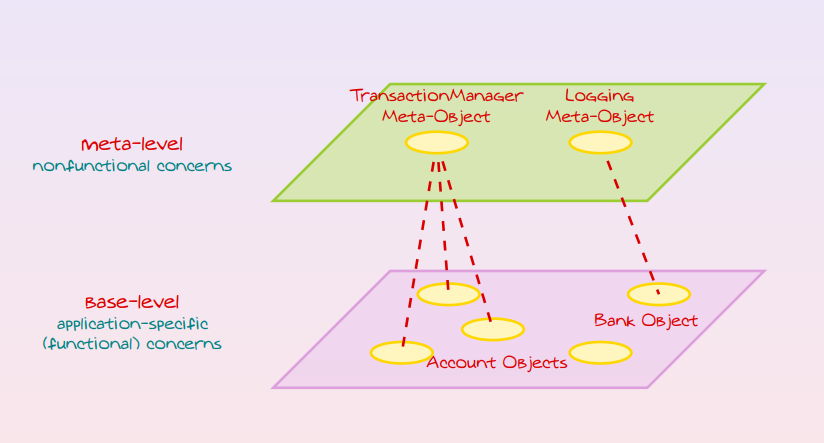
\includegraphics[scale=0.7]{7-separation-of-concerns-get-as-reflective-activity-contd}
\end{center}
















\section{Java Reflection}

\subsection{Reflection in Java}

\subsubsection{Introduction}

The \textbf{Java Core Reflection API} provides a small, type-safe, and secure API that supports introspection about the classes and objects in the current Java Virtual Machine.

\textbf{If permitted by security policy, the API can be used to}:
\begin{itemize}
	\item construct new class instances and new array
	\item access and modify fields of object and classes
	\item invoke methods on object and classes, and
	\item access and modify elements of array
\end{itemize}

Intercession on classes and objects is forbidden

\subsubsection{Introduction (Cont'd)}

\textbf{The Java application that benefint from introspection are}:

\begin{itemize}
	\item automatic documentation (javac, javadoc, ...)
	\item tools for IDEs: browsers, inspectors, debuggers, ...
	\item serialization / deserialization
	- construction of a binary representation for backup or transmission;
	- re-creating an object based on its serialized form;
	\item RMI
	- serialization of arguments and return values;
	- identification of remote methods.
\end{itemize}

\subsubsection{Classes and Interfaces for Reflection}

\textbf{Since Java <= 12}

- java.lang.Object
	- java.lang.Class
	- java.lang.reflect.Member
		
		- java.lang.reflect.Field (Member)
		- java.lang.reflect.Method (Member)
		- java.lang.reflect.Constructor (Member)

- boolean.class, char.class, int.class, double.class, ...




\section{Java Reflection}

\subsection{Reflection in Java}

\subsubsection{Introduction}

The \textbf{Java Core Reflection API} provides a small, type-safe, and secure API that supports introspection about the classes and objects in the current Java Virtual Machine.

\textbf{If permitted by security policy, the API can be used to}:
\begin{itemize}
	\item construct new class instances and new array
	\item access and modify fields of object and classes
	\item invoke methods on object and classes, and
	\item access and modify elements of array
\end{itemize}

Intercession on classes and objects is forbidden

\subsubsection{Introduction (Cont'd)}

\textbf{The Java application that benefint from introspection are}:

\begin{itemize}
	\item automatic documentation (javac, javadoc, ...)
	\item tools for IDEs: browsers, inspectors, debuggers, ...
	\item serialization / deserialization
	- construction of a binary representation for backup or transmission;
	- re-creating an object based on its serialized form;
	\item RMI
	- serialization of arguments and return values;
	- identification of remote methods.
\end{itemize}

\subsubsection{Classes and Interfaces for Reflection}

\textbf{Since Java < 12}

- java.lang.Object
	- java.lang.Class
	- java.lang.reflect.Member
		- java.lang.reflect.Field (Member)
		- java.lang.reflect.Method (Member)
		- java.lang.reflect.Constructor (Member)
		
- boolean.class, char.class, int.class, double.class, ...

\textbf{Since Java 13}

- java.lang.Object
	- java.lang.Class
	- java.lang.reflect.Member
	- java.lang.reflect.AccessibleObject
		- java.lang.reflect.Field (Member)
		- java.lang.reflect.Method (Member)
		- java.lang.reflect.Constructor (Member)
	- java.lang.reflect.Proxy
	- java.lang.reflect.InvocationHandler

- boolean.class, char.class, int.class, double.class, ...

\textbf{Since Java 15}

- java.lang.Object
	- java.lang.Class
	- java.lang.reflect.Member
	- java.lang.reflect.AccessibleObject
		- java.lang.reflect.Field (Member)
		- java.lang.reflect.Method (Member)
		- java.lang.reflect.Constructor (Member)
	- java.lang.reflect.Proxy
	- java.lang.reflect.InvocationHandler
	- java.lang.annotation.Annotation
	- java.lang.instrument.Instrumentation

boolean.class, char.class, int.class, double.class, ...

\subsubsection{The Java's Class Model}

%\begin{center}
%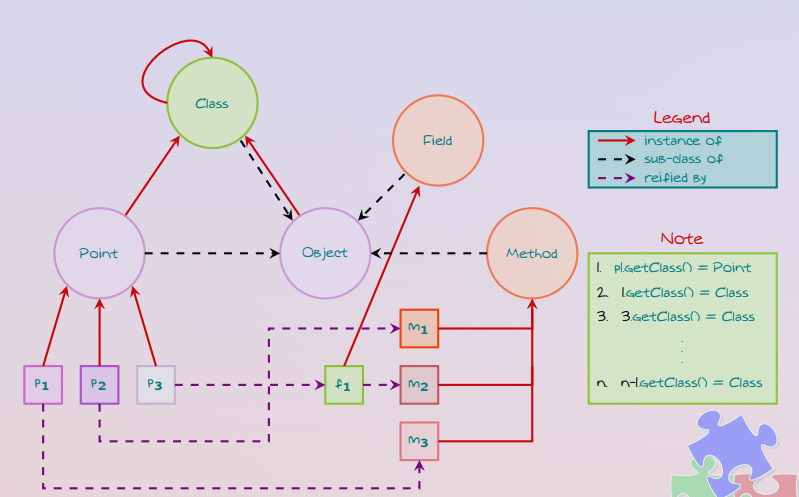
\includegraphics[scale=0.7]{8-the-javas-class-model}
%\end{center}

\subsubsection{Java's Limitations on Reflaction}

\textbf{The meta-object protocol is no causally connected}
	- Causal connectionposes a security rick, which has not been analyzed in the context of Java's bytecode verifier

\textbf{Class is declared final}
	- One cannot create new meta-classes
	
\textbf{There are no MOP operations to modify classes)}
	- Therefore, one cannot easily create and modularize class-to-class transformation
	
\textbf{Do the Java designers disagree with such transformtations? No}

\subsection{Java Reflection API (Package java.lang.reflect)}

\subsubsection{Class-to-Class Transformations: Marker Interfaces}

\textbf{Consider}
\begin{itemize}
	\item Clonable 
	\item Remote
	\item Serializable
\end{itemize}

Are these really interfaces? No

If not, what are they?
	- built-in class-to-class transformations

Java programmers cannot directly create such transformations

Other techniques must be employed ...
	- Some of them are the subject of the rest of this course

\subsubsection{Methods of Object}

\textbf{Object defines method to which all objects respond}

\begin{lstlisting}[language=Java]
class Object {
	public final Class<?> getClass() { ... }
	protected Object clone() { ... }
	public boolean equals(Object obj) { ... }
	public int hashcode() { ... }
	public String toString() { ... }
	public final void notify() { ... }
	public final void notifyAll() { ... }
	public final void wait() { ... }
		...
}
\end{lstlisting}

\subsubsection{Methods of Class<T>}

\textbf{Methods of Class<T>—Basic Operations}

\begin{lstlisting}[language=Java]
public final class Class<T> extends Object {
	public static Class<?> forName(String className) { ... }
	public static Class<?> forName(Module module, String name) { ... }
	public T newInstance() { ... } /* deprecated since 9 */
	public boolean isInstance(Object obj) { ... }
	public String getName() { ... }
	public Class<? super T> getSuperclass() { ... }
	public Module getModule() { ... }
	public Class<?>[] getInterfaces() { ... }
	public Class<?>[] getDeclaredClasses() throws SecurityException { ... }
	public Method[] getDeclaredMethods() throws SecurityException { ... }
	public Constructor<?> getEnclosingConstructor() throws SecurityException { ... }
	public Field[] getFields() throws SecurityException { ... }
		...
}
\end{lstlisting}

\subsubsection{java.lang.Class at Work}

\textbf{Let's write a method to return a printable class name}

\begin{lstlisting}[language=Java]
class MOP {
	public static String classNameToString(Class<?> cls) {
		if (!cls.isArray()) return cls.getName();
		else return cls.getComponentType().getName() + "[]";
	}
}
\end{lstlisting}

\begin{lstlisting}[language=Java]
[14:40]cazzola@hymir:~/tsp>jshell
| Welcome to JShell -- Version 11
| For an introduction type: /help intro
jshell> /open MOP1.java
jshell> MOP.classNameToString(String.class)
$2 ==> "java.lang.String"
jshell> var a = new Integer[]{1,2,3}
a ==> Integer[3] { 1, 2, 3 }
jshell> a.getClass()
$4 ==> class [Ljava.lang.Integer;
jshell> MOP.classNameToString(a.getClass())
$5 ==> "java.lang.Integer[]"
jshell> /exit
| Goodbye
\end{lstlisting}

\textbf{Let’s code a method to return super class hierarchy of a class}

\begin{lstlisting}[language=Java]
import java.util.ArrayList;
import java.util.List;

class MOP {
	public static Class<?>[] getAllSuperClasses(Class<?> cls) {
		List<Class<?>> result = new ArrayList<Class<?>>();
		for (Class<?> x = cls; x != null; x = x.getSuperclass()) result.add(x) ;
		return result.toArray(new Class<?>[0]);
	}
}
\end{lstlisting}

\begin{lstlisting}[language=Java]
[16:33]cazzola@hymir:~/tsp>jshell
jshell> /open MOP2.java
jshell> MOP.getAllSuperClasses(java.util.ArrayList.class)
$4 ==> Class[4] { class java.util.ArrayList, class java.util.AbstractList,
                  class java.util.AbstractCollection, class java.lang.Object }
\end{lstlisting}

\subsubsection{Summary for Class<T> Methods}

\textbf{Member Access}

getAnnotations
getAnnotation
getClasses
getConstructors
getConstructor
getDeclaredAnnotation
getDeclaredClasses
getDeclaredConstructors
getDeclaredConstructor
getDeclaredFields
getDeclaredField
getDeclaredMethods
getDeclaredMethod
getFields
getField
getMethods
getMethod

\textbf{Class Properties}

getComponentType
getDeclaringClass
getEnclosingClass
getEnclosingConstructor
getEnclosingMethod
getModifiers
isAnnotationPresent
isAnnotation
isAnonymousClass
isArray
isAssignableFrom
isEnum
isInterface
isPrimitive

\textbf{Context Access}

getClassLoader
getInterfaces
getModule
getPackage
getProtectionDomain
getResourceAsStream
getResource
getSigners

\subsubsection{Classes in java.lang.reflect}

%\begin{center}
%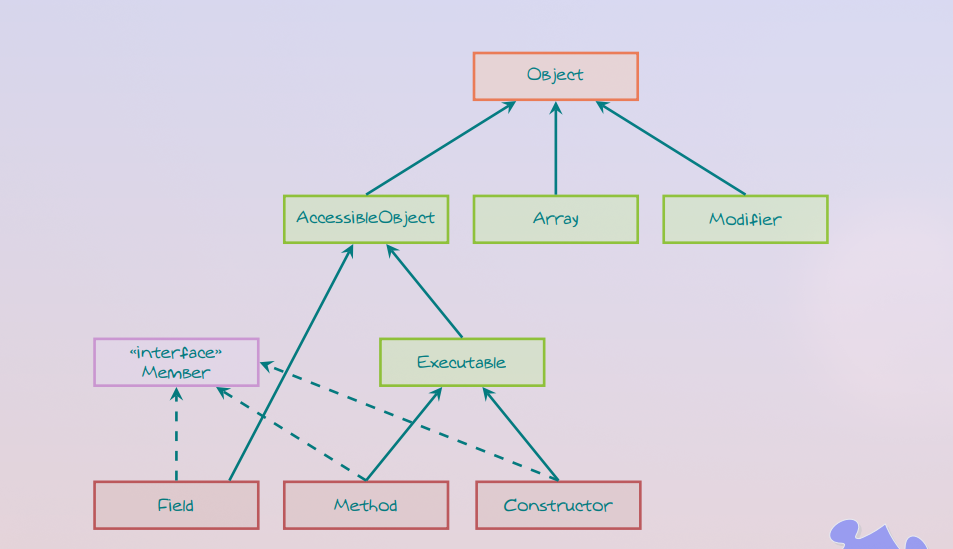
\includegraphics[scale=0.7]{9-classes-in-java-lang-reflected}
%\end{center}

Instances of Field, Constructor, and Method are meta-objects

\subsubsection{java.lang.reflect.Method}

\begin{lstlisting}[language=Java]
public final class Method extends Executable implements Member {
	public Class<?> getReturnType() { ... }
	public Class<?>[] getParameterTypes() { ... }
	public Class<?>[] getExceptionTypes() { ... }
	public Object invoke(Object obj, Object... args) throws IllegalAccessException,
		IllegalArgumentException, InvocationTargetException { ... }
			...
}
\end{lstlisting}

\subsubsection{When using invoke:}

\begin{itemize}
	\item individual parameters are automatically unwrapped to match primitive formal parameters, and
	\item both primitive and reference parameters are subject to method
invocation conversions as necessary.
\end{itemize}

\textbf{The return type is automatically wrapped in an Object}

\begin{lstlisting}[language=Java]
import java.util.stream.*;
import java.util.Arrays;
import java.lang.reflect.Method;

class MOP {
	public static String headerSuffixToString(Method m) {
		String result = MOP.classNameToString( m.getReturnType() ) + " " + m.getName()
				+ "(" + MOP.formalParametersToString( m ) + ")";
		Class<?>[] exs = m.getExceptionTypes();
		if (exs.length > 0) result += " throws " + MOP.classArrayToString(exs);
		return result;
	}
}
\end{lstlisting}

\begin{lstlisting}[language=Java]
[20:28]cazzola@hymir:~/tsp>jshell
jshell> /open MOP4.java
jshell> var cls = Class.forName("java.lang.reflect.Method")
cls ==> class java.lang.reflect.Method
jshell> var ms = Arrays.asList(cls.getDeclaredMethods()).stream()
	.filter(s->s.getName()=="invoke")
ms ==> java.util.stream.ReferencePipeline$2@548e7350
jshell> ms.forEach(m -> System.out.println(MOP.headerSuffixToString(m)))
java.lang.Object invoke(java.lang.Object p1, java.lang.Object[] p2)
	throws java.lang.IllegalAccessException, java.lang.IllegalArgumentException,
	java.lang.reflect.InvocationTargetException
\end{lstlisting}

\subsubsection{java.lang.reflect.Field}

\begin{lstlisting}[language=Java]
public final class Field extends AccessibleObject implements Member {
	public Class<?> getType() { ... };
	public Object get(Object obj)
		throws IllegalArgumentException, IllegalAccessException { ... };
	public void set(Object obj, Object value)
		throws IllegalArgumentException, IllegalAccessException { ... };
	public Class<?> getDeclaringClass() {...} ;
		... // Include get* and set* for the eight primitive types
}
\end{lstlisting}

\subsubsection{java.lang.reflect.AccessibleObject}

\textbf{Purpose}
It is the base class for Field, Method and Constructor objects
	- In this last two cases inherited by the Executable class.

It enables the suppression of the access control checks when:
\begin{itemize}
	\item setting or getting fields (using Field)
	\item invoking methods (using Method)
	\item  creating and initializing new instances of classes (Constructor)
\end{itemize}

\begin{lstlisting}[language=Java]
public final class AccessibleObject {
	public void setAccessible(boolean flag) throws SecurityException { ... }
	public static void setAccessible(AccessibleObject[] array, boolean flag)
			throws SecurityException { ... }
	public boolean isAccessible() { ... }
}
\end{lstlisting}

\textbf{Note that the Java security manager can forbid the use of setAccessible()}

\subsubsection{java.lang.reflect.AccessibleObject (Cont'd)}

\begin{lstlisting}[language=Java]
import java.lang.reflect.Field;

class Employee {
	private String name;
	public Employee(String name) { this.name = name; }
}

class AccessibilityCheck {
	public static void main(String[] args) {
		try {
			Employee mike = new Employee("Mike");
			Field name = Employee.class.getDeclaredField("name");
			name.setAccessible(true);
			System.out.println("Value of name: "+ name.get(mike));
			name.set(mike, "Eleonor");
			System.out.println("Changed value of name: " + name.get(mike));
		} catch(NoSuchFieldException | SecurityException | IllegalAccessException e) {
			System.out.println(e.getMessage());
		}
	}
}
\end{lstlisting}

\begin{lstlisting}[language=Java]
grant {
	permission java.lang.reflect.ReflectPermission
	"suppressAccessChecks";
};
\end{lstlisting}

\begin{lstlisting}[language=Java]
[22:53]cazzola@hymir:~/tsp>java AccessibilityCheck
Value of name: Mike
Changed value of name: Eleonor
[23:02]cazzola@hymir:~/tsp>java -Djava.security.manager AccessibilityCheck
access denied ("java.lang.reflect.ReflectPermission" "suppressAccessChecks")
[23:03]cazzola@hymir:~/tsp>java -Djava.security.policy=granted.policy
                                -Djava.security.manager AccessibilityCheck
Value of name: Mike
Changed value of name: Eleonor
\end{lstlisting}

\subsubsection{java.lang.reflect.Constructor}

\begin{lstlisting}[language=Java]
public final class Constructor extends AccessibleObject implements Member {
	public T newInstance(Object... initargs)
		throws InstantiationException, IllegalAccessException,
			IllegalArgumentException, InvocationTargetException { ... }
	...
}
\end{lstlisting}

\textbf{Note that newInstance() of Class invokes default constructor, other constructor are invoked with newInstance() of Constructor}

\subsubsection{Examples: Smart Reflective Access to Fields}

\begin{lstlisting}[language=Java]
import java.lang.reflect.*;

public interface SmartFieldAccess {
	default public Object instVarAt(String name) throws Exception {
		Field f = this.getClass().getDeclaredField(name);
		f.setAccessible(true);
		if (!Modifier.isStatic(f.getModifiers())) return f.get(this);
		return null;
}

default public void instVarAtPut(String name, Object value) throws Exception {
	Field f = this.getClass().getDeclaredField(name);
	f.setAccessible(true);
	if (!Modifier.isStatic(f.getModifiers())) f.set(this, value);
	}
}

class Employee implements SmartFieldAccess {
	private String name;
	public Employee(String name) {this.name=name;}
}
\end{lstlisting}

\begin{lstlisting}[language=Java]
[0:24]cazzola@hymir:~/tsp>jshell
jshell> /open SmartFieldAccess.java
jshell> var mike = new Employee("Mike");
mike ==> Employee@59f99ea
jshell> mike.instVarAtPut("name", "Eleonor")
jshell> mike.instVarAt("name")
$6 ==> "Eleonor"
\end{lstlisting}

\subsubsection{Examples: Reflective Cloning}

\begin{lstlisting}[language=Java]
import java.lang.reflect.Field;

public interface ReflectiveCloning {
	default public Object copy() throws Exception {
		Object tmp = this.getClass().getDeclaredConstructor().newInstance() ;
		Field[] fields = this.getClass().getDeclaredFields();
		for (int i = 0; i < fields.length; i++) {
			fields[i].setAccessible(true);
			fields[i].set(tmp, fields[i].get(this));
		}
		return tmp;
	}
}

class Employee implements ReflectiveCloning {
	private String name;
	public Employee() {this.name="Anon"; }
	public Employee(String name) {this.name=name;}
	public String toString() {return "Employee: "+this.name;}
}
\end{lstlisting}

\begin{lstlisting}[language=Java]
[1:04]cazzola@hymir:~/tsp>jshell
jshell> /open ReflectiveCloning.java
jshell> var e = new Employee("Mike");
e ==> Employee: Mike
jshell> var e1 = e.copy();
e1 ==> Employee: Mike
\end{lstlisting}

\subsubsection{Examples: Reflective Cloning}

\begin{lstlisting}[language=Java]
import java.lang.reflect.Method;

public interface SmartMessageSending {
	default public Object receive(String selector, Object[] args) throws Exception {
		Method mth = null; Class<?>[] classes = null;
		if (args != null) {
			classes = new Class<?>[args.length];
			for (int i = 0; i < args.length; i++) classes[i] = args[i].getClass();
		}
		mth = this.getClass().getMethod(selector, classes);
		return mth.invoke(this, args);
	}
}

class Employee implements SmartMessageSending {
	private String name;
	public Employee(String name) {this.name=name;}
	public void setName(String name) {this.name=name;}
	public String getName() {return this.name;}
	public String toString() {return "Employee: "+this.name;}
}
\end{lstlisting}

\begin{lstlisting}[language=Java]
jshell> var e = new Employee("Mike");
e ==> Employee: Mike
jshell> e.receive("getName", null)
$1 ==> "Mike"
jshell> e.receive("setName", new Object[]{"Eleonor"})
$2 ==> null
jshell> e
e ==> Employee: Eleonor
\end{lstlisting}

\subsection{Conclusions}

\textbf{Benefits}
\begin{itemize}
	\item reflection in Java opens up the structure and the execution trace of the program
	\item the reflective API is simple and quite complete
\end{itemize}

\textbf{Drawbacks}
\begin{itemize}
	\item reflection in Java is limited to introspection
	\item there isn’t a clear separation between the two logical layers (baseand meta-level)
	\item reflection in Java has been proved inefficient
\end{itemize}
\section{Java Annotations}

\subsection{Java Annotations}

\subsubsection{Meta-Data: What, Why and How}

\textbf{Annotations}, also called \textbf{meta-data}, are:

Data about the program execution can be introspected as well:
\begin{itemize}
	\item structured data that describe, explain, locate or make easier to retrieve, use or manage an information resource
\end{itemize}

Annotations are information about information that are interpreted at some point by code or data analysis tools.

Annotations can be used to:
\begin{itemize}
	\item document the code
	\item extract some specific data from the program (e.g., lint, metrics, and so on);
	\item automatically generate configuration files
	\item ...
\end{itemize}

\subsubsection{Meta-Data: A New Concept?}

Do annotations facility introduce a new concept in Java?

No, many applications require or produce files associated to a
specific class,

\begin{itemize}
	\item JAX-RPC, XML-RPC, SOAP, . . . ;
	\item EJB, JavaBean “BeanInfo” class
	\item ...
\end{itemize}

Creating and maintaining these associated files is painful.

Moreover many API need the use of special “placemarkers” 

Remote, Serializable, Cloneable, ... 

This feature adds a customizable mechanism for annotating classes, methods and fields

\subsubsection{Standard Annotations}

Standard annotation types are those provided "out-of-the-box"

\begin{itemize}
	\item \textbf{@Override}, to mark that a method overrides another method in its superclass
	\item \textbf{@Deprecated}, to indicate that the use of this method is discouraged; and
	\item \textbf{@SuppressWarning}, to turn off compiler warning for classes, methods, or field and variable initializers.
\end{itemize}

\begin{lstlisting}[language=Java]
@Override
public String toString() {
	return super.toString() + "[modified by subclass]" ;
}
\end{lstlisting}

\subsubsection{Categories of Custom Annotations}
There are three categories of custom annotations:
\begin{itemize}
	\item Marker Annotations, these are annotations without parameters or that uses default values for all parameters.
\begin{lstlisting}[language=Java]
@MarkerAnnotation
\end{lstlisting}	
	\item Single-Value Annotations, the annotations of this kind have just a single member named value
\begin{lstlisting}[language=Java]
@SingleValueAnnotation("some value");
\end{lstlisting}
	\item Full Annotations, these annotations exploits the full range of the annotation syntax
\begin{lstlisting}[language=Java]
@RevieVws({ // curly braces indicate an array of values
	@Review(grade=Review.Grade.EXCELLENT, reviewer="DF"),
	@Review(grade=Review.Grade.UNSATISFACTORY, reviewer="EG",
		comment="This method needs and @Override annotation.")
})
\end{lstlisting}
\end{itemize}

\subsubsection{Creating Custom Annotation Types}

Annotation types are, basically, Java interfaces
\begin{itemize}
	\item They look similar to a normal Java interface definition, but you use @interface which tells the compiler that you are writing an annotation type
\end{itemize}

Annotations’ members are defined by method signatures
\begin{itemize}
	\item these do not take any input parameters
	\item the return type defines the type of the member
\end{itemize}

\begin{lstlisting}[language=Java]
public @interface TODO {
	String value();
}
@TODO("Figure out the amount of interest per month")
	public void calculateInterest(float amount, float rate) {
	// need to finish this method later
}
\end{lstlisting}

Actually
\begin{itemize}
	\item when you write the method signature
	\item the compiler adds a member to the annotation with the same name and type after the method return type
	\item the method will be the selector for such a member
\end{itemize}

\subsubsection{Creating Custom Annotation Types (Cont'd)}

Similatly, we can define  annotation types with several members

\begin{lstlisting}[language=Java]
public @interface GroupTODO {
	public enum Severity {CRITICAL, IMPORTANT, TRIVIAL, DOCUMENTATION};
	Severity severity() default Severity.IMPORTANT;
	String item();
	String assignedTo();
}
@GroupTODO(
	severity=GroupTODO.Severity.CRITICAL,
	item="Figure out the amount of interest per month",
	assignedTo="Walter Cazzola"
)
public void calculateInterest(float amount, float rate) {
	// need to finish this method later
}
\end{lstlisting}

By omitting severity the default value would be used.


\subsubsection{Meta-Annotations, i.e., Annotations on Annotations}

The \textbf{meta-annotations} are annotations on annotations

There are four kind of predefined meta-annotations:

\begin{itemize}
	\item @Target, specifies which program elements (types, methods, ...) can have annotations of the defined type
	\item  @Retention, indicates whether an annotation is tossed out by the compiler or retained in the compiled class file.
	\item @Documented, indicates that the annotation should be considered as part of the public API of the annotated program element.
	\item @Inherited, is used on annotation types targeted at classes and indicates that the annotated type is an inherited one
\end{itemize}

\subsubsection{Reflecting on Annotations}

The easiest way to check for an annotation is by using the isAnnotationPresent() method.

\begin{lstlisting}[language=Java]
import java.lang.annotation.RetentionPolicy ;
import java.lang.annotation.Retention ;

@Retention(RetentionPolicy.RUNTIME)
public @interface TODO {
	String value();
}
\end{lstlisting}

\begin{lstlisting}[language=Java]
@TODO("Everything is still missing")
class Test {}
public class TestIsAnnotated {
	public static void main(String[] args) {
		Class c = Test.class;
		boolean todo = c.isAnnotationPresent(TODO.class);
		if (todo) System.out.println("The Test class is not completely implemented yet");
		else System.out.println("The Test class is completely implemented");
	}
}
\end{lstlisting}

\begin{lstlisting}[language=Java]
[23:01]cazzola@hymir:~/tsp>java TestIsAnnotated
The Test class is not completely implemented yet
\end{lstlisting}

\subsubsection{Reflecting on Annotations}

You can get the annotation’s members through its reification

\begin{lstlisting}[language=Java]
import java.lang.reflect.Method ;
class Test {
	@GroupTODO(
		severity=GroupTODO.Severity.CRITICAL,
		item="Figure out the amount of interest per month",
		assignedTo="Walter Cazzola")
	public void calculateInterest(float amount, float rate) {
		// need to finish this method later
	}
}
public class GetMembers {
	public static void main(String[] args) throws NoSuchMethodException {
	Class c = Test.class;
	Method element = c.getMethod("calculateInterest", float.class, float.class);
	GroupTODO groupTodo = element.getAnnotation(GroupTODO.class);
	String assignedTo = groupTodo.assignedTo();
	System.out.println("TODO item on Test is assigned to: '"+assignedTo+"'.");
	}
}
\end{lstlisting}
\section{Dynamic Proxy}

\subsection{Java's Dynamic Proxy}

\subsubsection{What Is a Proxy?}

The homonym design pattern defines a proxy as an:

\begin{itemize}
	\item object providing a surrogate/placeholder for another object
	\item to control and manipulate the accesses to it
\end{itemize}

Few examples

\begin{itemize}
	\item local representation of remote objects;
	\item delay of expensive operations;
	\item access protection for secure objects.
\end{itemize}

\subsubsection{What Is a Dyniamic Proxy?}

A dynamic proxy class is a class implementing a \textbf{list of interfaces} such that the invocation of a method beloging to one of these interfaces on one of its instances is \textbf{seamleassly dispatched} to another object implementing such interface and bound to the dynamic proxy object.

A dynamic proxy class can be used to create a type-safe proxy object for a set of objects determined by the implemented interfaces \textbf{without} both \textbf{explicit coding} and \textbf{static pre generation} of the proxy class as happens with several compile-time tools.

Dynamic proxy classes are useful to applications or libraries that need to provide type-safe reflective dispatch of invocations on objects whose interface is available

java.lang.reflect.InvocationHandler

\subsubsection{java.lang.reflect.InvocationHandler}

Each proxy instance has an associated invocation handler.

When a method is invoked on a proxy instance

\begin{itemize}
	\item the method invocation is dispatched to the invoke() method of its invocation handler
\end{itemize}

\begin{center}
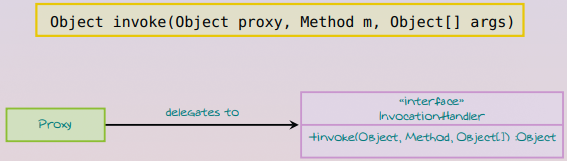
\includegraphics[scale=0.7]{10-invocation-handler}
\end{center}

\subsubsection{java.lang.reflect.Proxy}

Proxy

\begin{itemize}
	\item  provides static methods for creating dynamic proxy classes and instances, and
	\item  it also is the superclass of all dynamic proxy classes created by these methods
\end{itemize}

\begin{lstlisting}[language=Java]
public final class Proxy extends Object implements Serializable {
	protected InvocationHandler h;
	protected Proxy(InvocationHandler h) { ... }
	public static InvocationHandler getInvocationHandler(Object proxy) { ... }
	public static Class<?> getProxyClass(ClassLoader l, Class<?>... interfaces) { ... }
	public static boolean isProxyClass(Class<?> cl) { ... }
	public static Object newProxyInstance(ClassLoader loader, Class<?>[] interfaces, InvocationHandler h ) { ... }
}
\end{lstlisting}

Basically, Proxy enables the meta-object approach in Java

\subsubsection{How Java Creates a Proxy}

\begin{center}
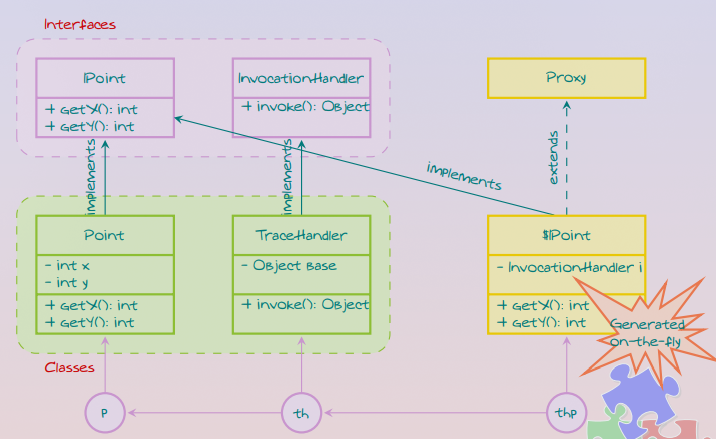
\includegraphics[scale=0.4]{11-create-a-proxy}
\end{center}

\subsubsection{Example: To Trace the Method Calls}

\begin{lstlisting}[language=Java]
import java.lang.reflect.*;
public class TraceHandler implements InvocationHandler {
	private Object baseObject;
	public TraceHandler(Object base) { baseObject = base; }
	public Object invoke(Object proxy, Method m, Object[] args) {
	try {
		System.out.println("before " + m.getName());
		Object result = m.invoke(baseObject, args);
		System.out.println("after " + m.getName());
		return result;
	} catch (Exception e) {
		e.printStackTrace(); 
		return null;
	}
}
public String toString() { return "th :- "+this.baseObject; }
}
\end{lstlisting}

\begin{lstlisting}[language=Java]
jshell> IPoint p1 = new Point(10,20);
p1 ==> p :- (10, 20)
jshell> IPoint th_p1 = (IPoint) Proxy.newProxyInstance(
p1.getClass().getClassLoader(), p1.getClass().getInterfaces(), new TraceHandler(p1));
before toString
after toString
th_p1 ==> p :- (10, 20)
jshell> p1.getX(); /* standard call */
$10 ==> 10
jshell> th_p1.getX(); /* traced call */
before getX
after getX
$11 ==> 10
\end{lstlisting}

\subsubsection{Example: Invariant Checking and Proxy Chaining}

\begin{lstlisting}[language=Java]
import java.lang.reflect.*;

public class InvariantHandler implements InvocationHandler {
	private Object target;
	private Method invariant;
	public InvariantHandler(Object target) {
		this.target = target;
		try {
			invariant = target.getClass().getMethod("invariant", new Class<?>[]{});
			if (!invariant.getReturnType().equals(boolean.class)) invariant = null;
		} 
		catch (NoSuchMethodException ex) { 
			invariant = null; }
		}
		
public Object invoke(Object proxy, Method method, Object[] args) throws Throwable {
	this.invokeInvariant(method);
	Object retvalue = method.invoke(this.target, args);
	this.invokeInvariant(method);
	return retvalue;
}

private void invokeInvariant(Method method) {
	if ((this.invariant == null) || (method.equals(this.invariant))) return;
	try {
		Boolean passed = (Boolean) invariant.invoke(target, new Object[]{});
		if (!passed.booleanValue()) throw new RuntimeException();
	} catch (Exception e) {
		System.out.println("Failed invariant check!!!"); 
	}
}
public String toString() {return "ih :- "+this.target; }
}
\end{lstlisting}

\subsubsection{Example: Invariant Checking and Proxy Chaining (Cont'd)}

\begin{lstlisting}[language=Java]
jshell> InvariantHandler ih = new InvariantHandler(new Point(0, 7));
ih ==> ih :- p :- (0, 7)
jshell> IPoint invariantCheckedPoint =
(IPoint)Proxy.newProxyInstance(
Point.class.getClassLoader(),
new Class[]{ IPoint.class }, ih);
invariantCheckedPoint ==> p :- (0, 7)
jshell> TraceHandler th = new TraceHandler(invariantCheckedPoint);
th ==> th :- p :- (0, 7)
jshell> IPoint tracedInvariantCheckedPoint =
(IPoint)Proxy.newProxyInstance(
Point.class.getClassLoader(),
new Class[] { IPoint.class }, th);
before toString
after toString
tracedInvariantCheckedPoint ==> p :- (0, 7)
jshell> tracedInvariantCheckedPoint.setX(25)
before setX
after setX
jshell> tracedInvariantCheckedPoint.setY(-7)
before setY
Failed invariant check!!!
after setY
\end{lstlisting}

\subsubsection{Example: Invariant Checking and Proxy Chaining (Cont'd)}

\begin{center}
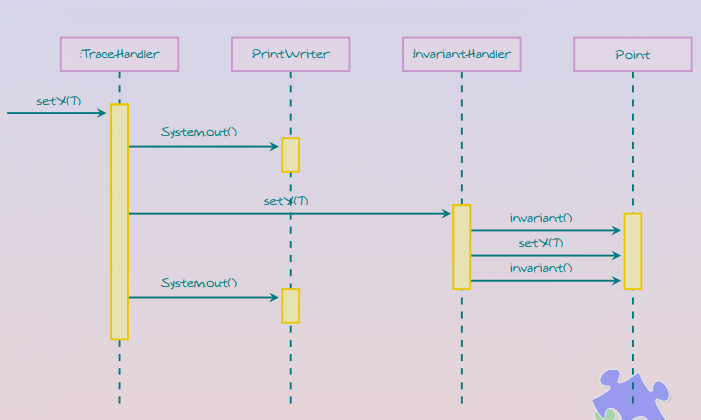
\includegraphics[scale=0.4]{12-proxy-chaining}
\end{center}



\section{Dynamic Proxy}

\subsection{Java's Dynamic Proxy}

\subsubsection{What Is a Proxy?}

The homonym design pattern defines a proxy as an:

\begin{itemize}
	\item object providing a surrogate/placeholder for another object
	\item to control and manipulate the accesses to it
\end{itemize}

Few examples

\begin{itemize}
	\item local representation of remote objects;
	\item delay of expensive operations;
	\item access protection for secure objects.
\end{itemize}

\subsubsection{What Is a Dyniamic Proxy?}

A dynamic proxy class is a class implementing a \textbf{list of interfaces} such that the invocation of a method beloging to one of these interfaces on one of its instances is \textbf{seamleassly dispatched} to another object implementing such interface and bound to the dynamic proxy object.

A dynamic proxy class can be used to create a type-safe proxy object for a set of objects determined by the implemented interfaces \textbf{without} both \textbf{explicit coding} and \textbf{static pre generation} of the proxy class as happens with several compile-time tools.

Dynamic proxy classes are useful to applications or libraries that need to provide type-safe reflective dispatch of invocations on objects whose interface is available

java.lang.reflect.InvocationHandler

\subsubsection{java.lang.reflect.InvocationHandler}

Each proxy instance has an associated invocation handler.

When a method is invoked on a proxy instance

\begin{itemize}
	\item the method invocation is dispatched to the invoke() method of its invocation handler
\end{itemize}

\begin{center}
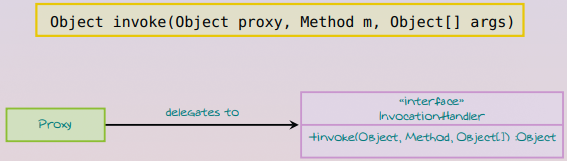
\includegraphics[scale=0.7]{10-invocation-handler}
\end{center}

\subsubsection{java.lang.reflect.Proxy}

Proxy

\begin{itemize}
	\item  provides static methods for creating dynamic proxy classes and instances, and
	\item  it also is the superclass of all dynamic proxy classes created by these methods
\end{itemize}

\begin{lstlisting}[language=Java]
public final class Proxy extends Object implements Serializable {
	protected InvocationHandler h;
	protected Proxy(InvocationHandler h) { ... }
	public static InvocationHandler getInvocationHandler(Object proxy) { ... }
	public static Class<?> getProxyClass(ClassLoader l, Class<?>... interfaces) { ... }
	public static boolean isProxyClass(Class<?> cl) { ... }
	public static Object newProxyInstance(ClassLoader loader, Class<?>[] interfaces, InvocationHandler h ) { ... }
}
\end{lstlisting}

Basically, Proxy enables the meta-object approach in Java

\subsubsection{How Java Creates a Proxy}

\begin{center}
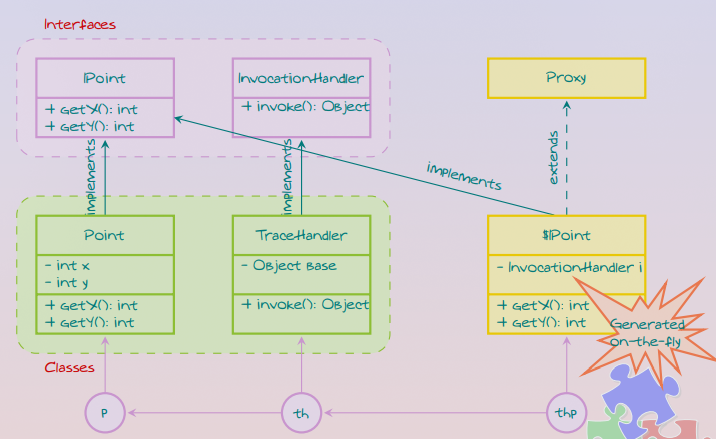
\includegraphics[scale=0.4]{11-create-a-proxy}
\end{center}

\subsubsection{Example: To Trace the Method Calls}

\begin{lstlisting}[language=Java]
import java.lang.reflect.*;
public class TraceHandler implements InvocationHandler {
	private Object baseObject;
	public TraceHandler(Object base) { baseObject = base; }
	public Object invoke(Object proxy, Method m, Object[] args) {
	try {
		System.out.println("before " + m.getName());
		Object result = m.invoke(baseObject, args);
		System.out.println("after " + m.getName());
		return result;
	} catch (Exception e) {
		e.printStackTrace(); 
		return null;
	}
}
public String toString() { return "th :- "+this.baseObject; }
}
\end{lstlisting}

\begin{lstlisting}[language=Java]
jshell> IPoint p1 = new Point(10,20);
p1 ==> p :- (10, 20)
jshell> IPoint th_p1 = (IPoint) Proxy.newProxyInstance(
p1.getClass().getClassLoader(), p1.getClass().getInterfaces(), new TraceHandler(p1));
before toString
after toString
th_p1 ==> p :- (10, 20)
jshell> p1.getX(); /* standard call */
$10 ==> 10
jshell> th_p1.getX(); /* traced call */
before getX
after getX
$11 ==> 10
\end{lstlisting}

\subsubsection{Example: Invariant Checking and Proxy Chaining}

\begin{lstlisting}[language=Java]
import java.lang.reflect.*;

public class InvariantHandler implements InvocationHandler {
	private Object target;
	private Method invariant;
	public InvariantHandler(Object target) {
		this.target = target;
		try {
			invariant = target.getClass().getMethod("invariant", new Class<?>[]{});
			if (!invariant.getReturnType().equals(boolean.class)) invariant = null;
		} 
		catch (NoSuchMethodException ex) { 
			invariant = null; }
		}
		
public Object invoke(Object proxy, Method method, Object[] args) throws Throwable {
	this.invokeInvariant(method);
	Object retvalue = method.invoke(this.target, args);
	this.invokeInvariant(method);
	return retvalue;
}

private void invokeInvariant(Method method) {
	if ((this.invariant == null) || (method.equals(this.invariant))) return;
	try {
		Boolean passed = (Boolean) invariant.invoke(target, new Object[]{});
		if (!passed.booleanValue()) throw new RuntimeException();
	} catch (Exception e) {
		System.out.println("Failed invariant check!!!"); 
	}
}
public String toString() {return "ih :- "+this.target; }
}
\end{lstlisting}

\subsubsection{Example: Invariant Checking and Proxy Chaining (Cont'd)}

\begin{lstlisting}[language=Java]
jshell> InvariantHandler ih = new InvariantHandler(new Point(0, 7));
ih ==> ih :- p :- (0, 7)
jshell> IPoint invariantCheckedPoint =
(IPoint)Proxy.newProxyInstance(
Point.class.getClassLoader(),
new Class[]{ IPoint.class }, ih);
invariantCheckedPoint ==> p :- (0, 7)
jshell> TraceHandler th = new TraceHandler(invariantCheckedPoint);
th ==> th :- p :- (0, 7)
jshell> IPoint tracedInvariantCheckedPoint =
(IPoint)Proxy.newProxyInstance(
Point.class.getClassLoader(),
new Class[] { IPoint.class }, th);
before toString
after toString
tracedInvariantCheckedPoint ==> p :- (0, 7)
jshell> tracedInvariantCheckedPoint.setX(25)
before setX
after setX
jshell> tracedInvariantCheckedPoint.setY(-7)
before setY
Failed invariant check!!!
after setY
\end{lstlisting}

\subsubsection{Example: Invariant Checking and Proxy Chaining (Cont'd)}

\begin{center}
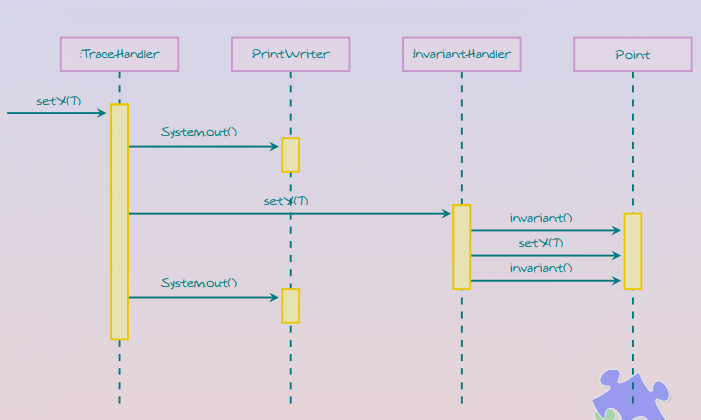
\includegraphics[scale=0.4]{12-proxy-chaining}
\end{center}


 

\section{Reflection vs Modules and Handles}

\subsection{Modules and Reflection}

\subsubsection{Private and Reflective Access}

\begin{lstlisting}[language=Java]
package tsp.module.employee;
import tsp.module.reflection.* ;
class Employee implements SmartFieldAccess {
	private String name;
	private String surname;
	public Employee(String n, String s) { this.name = n; this.surname = s; }
	public String toString() {return "Employee: "+this.name+" "+this.surname;}
}
\end{lstlisting}

\begin{lstlisting}[language=Java]
package tsp.module.reflection ;
import java.lang.reflect.*;
public interface SmartFieldAccess {
	default public Object instVarAt(String name) throws Exception {
		Field f = this.getClass().getDeclaredField(name);
		f.setAccessible(true);
		if (!Modifier.isStatic(f.getModifiers())) return f.get(this);
		return null;
	}

	default public void instVarAtPut(String name, Object value) throws Exception {
		Field f = this.getClass().getDeclaredField(name);
		f.setAccessible(true);
		if (!Modifier.isStatic(f.getModifiers())) f.set(this, value);
	}
}
\end{lstlisting}

\subsubsection{Private and Reflective Access (Cont'd).}

\begin{lstlisting}[language=Java]
package tsp.module.employee ;
public class ReflectiveEmployeeMain {
	public static void main(String[] args) throws Exception {
		Employee angela = new Employee("Angela", "Runedottir");
		System.out.println(angela);
		angela.instVarAtPut("surname", "Odindottir");
		System.out.println(angela);
	}
}
\end{lstlisting}

\begin{lstlisting}[language=Java]
[16:38]cazzola@hymir:~/tsp>java tsp.module.employee.ReflectiveEmployeeMain
Employee: Angela Runedottir
Employee: Angela Odindottir
\end{lstlisting}

\subsubsection{Modules: Whats, Whys and Hows}

Java 9 introduced the Java Module Platform.

Its goals are:

\begin{itemize}
	\item Reliable configuration, to replace the brittle, error-prone classpath mechanism in favor of a programming mechanism to explicitly declare dependencies
	\item Strong encapsulation, to allow a component to declare which of its public types are accessible to other components, and which are not.
\end{itemize}

A module:

\begin{itemize}
	\item groups classes, interfaces and packages
	\item a module-info.java file describes the dependencies between modules
\end{itemize}

\begin{lstlisting}[language=Java]
module com.foo.bar {
	requires org.baz.foo ;
	exports com.foo.bar.abc;
}
\end{lstlisting}

- the module-info.class file is shipped inside a jar file.

\subsubsection{Modules a New Obstacle to Reflection}

\begin{lstlisting}[language=Java]
module tsp.module.employee {
	requires tsp.module.reflection ;
	exports tsp.module.employee ;
}
\end{lstlisting}

\begin{lstlisting}[language=Java]
module tsp.module.reflection {
	exports tsp.module.reflection ;
}
\end{lstlisting}

\begin{lstlisting}[language=Java]
> javac tmr/module-info.java tmr/tsp/module/reflection/SmartFieldAccess.java
> javac --module-path=. tme/module-info.java tme/tsp/module/employee/*.java
> java --module-path . -m tme/tme.ReflectiveEmployeeMain
Employee: Angela Runedottir
Exception in thread "main" java.lang.reflect.InaccessibleObjectException: Unable to
make field private java.lang.String tme.Employee.surname accessible:
module tme does not "opens tme" to module tmr
...
at tmr/tmr.SmartFieldAccess.instVarAtPut(SmartFieldAccess.java:15)
at tme/tme.ReflectiveEmployeeMain.main(ReflectiveEmployeeMain.java:12)
\end{lstlisting}

Where:
- tmr stands for tsp.module.reflection, and
- tme stands for tsp.module.employee

\subsubsection{How to Get around Modules' Strong Encapsulation}

Several things can be done:

\begin{itemize}
	\item To pass -add-opens to the JVM to open the module
	- Isn’t always possible to pass a flag to the JVM, e.g., with frameworks0/tools that activate their own JVM.
	\item to open the
	- tme module to everyone,
	- tme package to everyone, or
	- tme package only to tmr
	\item in the corresponding module-info.java file
	- These options aren’t always applicable, e.g., in case of a too complex
project, when the module-info.java file is unavailable, . . .
\end{itemize}

Let’s see this last option

\subsubsection{Reflection Works Only on Open Modules}

\begin{lstlisting}[language=Java]
module tsp.module.employee {
	requires tsp.module.reflection ;
	exports tsp.module.employee ;
}
\end{lstlisting}

\begin{lstlisting}[language=Java]
module tsp.module.reflection {
	exports tsp.module.reflection ;
}
\end{lstlisting}

\begin{lstlisting}[language=Java]
> javac tmr/module-info.java tmr/tsp/module/reflection/SmartFieldAccess.java
> javac --module-path=. tme/module-info.java tme/tsp/module/employee/*.java
> java --module-path . -m tme/tme.ReflectiveEmployeeMain
Employee: Angela Runedottir
Employee: Angela Odindottir
\end{lstlisting}

Where:
- tmr stands for tsp.module.reflection, and
- tme stands for tsp.module.employee

\subsubsection{Module Graph}

The module system resolves the dependencies among modules by

\begin{itemize}
	\item locating observable modules to fulfill those dependencies, and then
	\item resolves the dependencies of these modules, and so forth
	\item until every dependency of every module is fulfilled.
\end{itemize}

This transitive-closure computation originates a module graph where each directed edge represents a fulfilled dependency among modules (the nodes).

\begin{lstlisting}[language=Java]
[23:40]cazzola@hymir:~/tsp>jdeps --module-path=. -m tme -summary -recursive
tsp.module.employee -> java.base
tsp.module.employee -> tsp.module.reflection
tsp.module.reflection -> java.base
\end{lstlisting}

\subsubsection{Reflecting on Modules}

\begin{lstlisting}[language=Java]
[23:52]cazzola@hymir:~/tsp> jshell --module-path=. --add-modules=tsp.module.employee
--add-exports=tsp.module.employee/tsp.module.employee:jshell
jshell> import tsp.module.reflection.* ;
jshell> import tsp.module.employee.* ;
jshell> Module myClassModule = Employee.class.getModule();
myClassModule ==> module tsp.module.employee
jshell> myClassModule.isNamed();
$1 ==> true
jshell> import java.lang.module.*;
jshell> ModuleDescriptor descriptor = myClassModule.getDescriptor();
descriptor ==> module {name:tsp.module.employee, [mandated ... [tsp.module.reflection]]}
jshell> descriptor.toString();
$2 ==> "module { name: tsp.module.employee,
[mandated java.base (@11), tsp.module.reflection],
exports: [tsp.module.employee],
opens: [tsp.module.employee to [tsp.module.reflection]] }"
jshell> ModuleDescriptor d2 = SmartFieldAccess.class.getModule().getDescriptor() ;
d2 ==> module { name: tsp.module.reflection, [mandated j ...
[tsp.module.reflection] }
jshell> d2.toString();
$3 ==> "module { name: tsp.module.reflection,
[mandated java.base (@11)], exports: [tsp.module.reflection] }"
jshell> descriptor.exports();
$4 ==> [tsp.module.employee]
jshell> descriptor.packages();
$5 ==> [tsp.module.employee]
\end{lstlisting}

\subsubsection{Privates Are Not So Private}

\begin{lstlisting}[language=Java]
import java.lang.invoke.MethodHandles.*;
class Employee implements SmartFieldAccess {
	private final Lookup lookup;
	public Lookup getEmployeeLookup() {return this.lookup;}
	private String name; private String surname;
	public Employee(String n, String s){lookup=MethodHandles.lookup(); name=n; 			surname=s;}
}
\end{lstlisting}

\begin{lstlisting}[language=Java]
import java.lang.invoke.*;
import java.lang.invoke.MethodHandles.*;
public interface SmartFieldAccess {
	default public Object instVarAt(Lookup lookup, String name) throws Exception {
		Class<?> clazz = this.getClass();
		Field f = clazz.getDeclaredField(name);
		MethodHandles.Lookup privateLookup = MethodHandles.privateLookupIn(clazz, lookup);
		VarHandle handle = privateLookup.unreflectVarHandle(f);
		if (!Modifier.isStatic(f.getModifiers())) return handle.get(this);
		return null;
	}
	default public void instVarAtPut(Lookup lookup, String n, Object v) throws Exception{
		Class<?> clazz = this.getClass();
		Field f = clazz.getDeclaredField(n);
		MethodHandles.Lookup privateLookup = MethodHandles.privateLookupIn(clazz, lookup);
		VarHandle handle =  privateLookup.unreflectVarHandle(f);
		if (!Modifier.isStatic(f.getModifiers())) handle.set(this, v);
	}
}
\end{lstlisting}


\subsubsection{Privates Are Not So Private (Cont'd)}

\begin{lstlisting}[language=Java]
package tsp.module.employee ;

public class GlasnotEmployeeMain {
	public static void main(String[] args) throws Exception {
		Employee angela = new Employee("Angela", "Runedottir");
		System.out.println(angela);
		angela.instVarAtPut(angela.getEmployeeLookup(), "surname", "Odindottir");
		System.out.println(angela);
	}
}
\end{lstlisting}

\begin{lstlisting}[language=Java]
> javac tmr/module-info.java tmr/tsp/module/reflection/SmartFieldAccess.java
> javac --module-path=. tme/module-info.java tme/tsp/module/employee/*.java
> java --module-path . -m tme/tme.GlasnotEmployeeMain
Employee: Angela Runedottir
Employee: Angela Odindottir
\end{lstlisting}

where:
- tmr stands for tsp.module.reflection, and
- tme stands for tsp.module.employee

\subsubsection{Variable Handles}

A variable handle is a typed reference to a variable:

\begin{itemize}
	\item VarHandle class provides read/write access to variables
	\item VarHandles are immutable and have no visible state
\end{itemize}

Each VarHandle has:

\begin{itemize}
	\item a variable type T that corresponds to the type of the variable
	\item abstracts the safe access to a memory location
	\item a list of coordinate types CT1. CT2, . . . , CTn
\end{itemize}

\begin{lstlisting}[language=Java]
Factory methods to produce/lookup VarHandles:
MethodHandles.lookup().in(Foo.class).findVarHandle(Foo.class, "i", int.class);
\end{lstlisting}

\begin{lstlisting}[language=Java]
MethodHandles.privateLookupIn(Foo.class, MethodHandles.lookup())
.findVarHandle(Foo.class, "i", int.class);
\end{lstlisting}

\subsubsection{Access modes}
\begin{itemize}
	\item read, e.g., get, getVolatile, ...
	\item write, e.g., set, setOpaque, ...
	\item atomic update, compareAndSet, getAndSet, ...
\end{itemize}
\end{document}
